\documentclass{article}




\usepackage{geometry}
\usepackage{amsmath}
\usepackage{graphicx}
\usepackage{listings}
\usepackage{xcolor}
\usepackage{chngcntr}


\geometry{letterpaper, margin=1.5in, bottom=1in}

\counterwithin*{equation}{subsection}

\title{Problem Set One}
\date{02/07/2018}
\author{Zhixian(Jason) Yu}

\definecolor{mygreen}{rgb}{0,0.6,0}
\definecolor{mygray}{rgb}{0.9,0.9,0.9}
\definecolor{mymauve}{rgb}{0.58,0,0.82}

\lstset{ %
  backgroundcolor=\color{mygray},   % choose the background color
  basicstyle=\footnotesize,        % size of fonts used for the code
  breaklines=true,                 % automatic line breaking only at whitespace
  captionpos=b,                    % sets the caption-position to bottom
  commentstyle=\color{mygreen},    % comment style
  escapeinside={\%*}{*)},          % if you want to add LaTeX within your code
  keywordstyle=\color{blue},       % keyword style
  stringstyle=\color{mymauve},     % string literal style
  keepspaces=true,
  tabsize=2,
  language=Python,
  numbersep=3pt, 
  numbers=left
  %frame=single
}

\begin{document}
\maketitle
\pagenumbering{gobble}
\newpage

\section{Theory}
\subsection{}
The coordinates w.r.t. the Walsh basis is:
\begin{equation*}
{U_1}^{-1} x = 
\left[\begin{matrix}
1 & 1 & 1 & 1 \\
1 & 1 & -1 & -1 \\
1 & -1 & -1 & 1 \\
1 & -1 & 1 & -1
\end{matrix}
\right]
\left[\begin{matrix}
0 \\
0 \\
1 \\
-1
\end{matrix}
\right] = \begin{bmatrix}
0\\
0\\
-2\\
2
\end{bmatrix}
\end{equation*}
The coordinates w.r.t. the Haar basis is:
\begin{equation*}
{U_2}^{-1} x = \frac{1}{2}
\left[\begin{matrix}
1 & 1 & 1 & 1 \\
1 & 1 & -1 & -1 \\
\sqrt{2} & -\sqrt{2} & 0 & 0 \\
0 & 0 & \sqrt{2} & -\sqrt{2}
\end{matrix}
\right]
\left[\begin{matrix}
0 \\
0 \\
1 \\
-1
\end{matrix}
\right] = \begin{bmatrix}
0\\
0\\
0\\
\sqrt{2}
\end{bmatrix}
\end{equation*}
It is better to project on the Haar basis because the basis vector $\left[\begin{matrix}
0 & 0 & \sqrt{2} & -\sqrt{2} \end{matrix}\right]^T$ captures all the variance of this point.


\subsection{}
Suppose the representation of $x$ in the 2D subspace w.r.t. the basis for $U$ is $\hat{x}$. Therefore the projection of $x$ onto the subspace spanned by $U$ is $U\hat{x}$, and the novelty of this point is $(x-U\hat{x})$.\\
Since the novelty is orthogonal to vectors of $U$, we have:
\begin{equation}
\label{eq:1.2}
U^T(x-U\hat{x}) = 0
\end{equation}
We can rewrite equation~\ref{eq:1.2} as:
\begin{equation}
U^T x = U^T U \hat{x}
\end{equation}
Therefore:
\begin{equation}
\hat{x} = (U^TU)^{-1} U^T x
\end{equation}
Solving this gives us $\hat{x}$, and $
\hat{x} = 
\begin{bmatrix}
5 \\ 5
\end{bmatrix}$.\\
The projection of the point onto subspace spanned by U is$
\begin{bmatrix}
2.5 \\
2.5 \\
0 \\
0
\end{bmatrix}$,
and the novelty is $
\begin{bmatrix}
-0.5 \\
0.5 \\
1 \\
-1
\end{bmatrix}$.


\subsection{}
The goal is to find an orthonormal matrix $Q$ and an upper triangular matrix $R$ so that $X=QR$ where $X=\begin{bmatrix}
0 & 1 & 1 \\
-1 & -2 & 2 \\
-1 & 3 & 3
\end{bmatrix}$. Here the vectors of $X$ were reordered for calculation purpose.\\
In the following calculation, $X_i$ denotes the ith column vector of $X$, $Q_i$ denotes the ith column vector of $Q$, and $R_{ij}$ denotes the ith row, jth column of R. \\
\begin{align*}
R_{11} &= \|{X_1}\| = \sqrt{2} \\
Q_1 &= \frac{X_1}{\|{X_1}\|} = \begin{bmatrix}0 \\ -\frac{\sqrt{2}}{2} \\[0.5em] -\frac{\sqrt{2}}{2}\end{bmatrix} \\
R_{12} &= {X_2}^T Q_1 = -\frac{\sqrt{2}}{2} \\
\overset{\sim}{Q_2} &= X_2 - R_{12}Q_1 = \begin{bmatrix}1 \\ -\frac{5}{2} \\[0.5em] \frac{5}{2}\end{bmatrix} \\
R_{22} &= \|\overset{\sim}{Q_2}\| = \frac{\sqrt{54}}{2} \\
Q_2 &= \frac{\overset{\sim}{Q_2}}{\|{\overset{\sim}{Q_2}}\|} = \begin{bmatrix}\frac{2}{\sqrt{54}} \\[0.5em] -\frac{5}{\sqrt{54}} \\[0.5em] \frac{5}{\sqrt{54}}\end{bmatrix} \\
R_{13} &= {X_3}^T Q_1 = -\frac{5\sqrt{2}}{2} \\
R_{23} &= {X_3}^T Q_2 = \frac{7}{\sqrt{54}} \\
\overset{\sim}{Q_3} &= X_3 - R_{13}Q_1 - R_{23}Q_2 = \begin{bmatrix}\frac{20}{27} \\[0.5em] \frac{4}{27} \\[0.5em] -\frac{4}{27}\end{bmatrix} \\
R_{33} &= \|\overset{\sim}{Q_3}\| = \frac{12\sqrt{3}}{27} \\
Q_3 &= \frac{\overset{\sim}{Q_3}}{\|{\overset{\sim}{Q_3}}\|} = \begin{bmatrix}\frac{5}{3\sqrt{3}} \\[0.5em] \frac{1}{3\sqrt{3}} \\[0.5em] -\frac{1}{3\sqrt{3}}\end{bmatrix}
\end{align*}
The final results are:
\begin{align*}
Q &= \begin{bmatrix}
0                   & \frac{2}{3\sqrt{6}}  & \frac{5}{3\sqrt{3}} \\[0.5em]
-\frac{\sqrt{2}}{2} & -\frac{5}{3\sqrt{6}} & \frac{1}{3\sqrt{3}} \\[0.5em]
-\frac{\sqrt{2}}{2} & \frac{5}{3\sqrt{6}}  & -\frac{1}{3\sqrt{3}}
\end{bmatrix}\\
R &= \begin{bmatrix}
\sqrt{2} & -\frac{\sqrt{2}}{2}  & -\frac{5\sqrt{2}}{2} \\[0.5em]
0        & \frac{3\sqrt{6}}{2} & \frac{7}{3\sqrt{6}} \\[0.5em]
0        & 0  & \frac{12\sqrt{3}}{27}
\end{bmatrix}
\end{align*}
And:
\begin{equation*}
Q^T Q = I
\end{equation*}


\subsection{}
Assume C is a symmetric matrices, we have:
\begin{equation}
\label{eq:base1}
C = C^*
\end{equation}

\paragraph{a)} To prove the eigenvalues are real, let $\lambda$ is any eigenvalue and $u$ is the associated eigenvector. We have:
\begin{equation}
\label{eq:real_eval_base2}
Cu = \lambda u
\end{equation}
From equation~\ref{eq:real_eval_base2}, we have:
\begin{equation}
\label{eq:real_eval_times_transpose}
u^*Cu = u^* \lambda u
\end{equation}
If we take the conjugate transpose for both sides of equation~\ref{eq:real_eval_times_transpose}, we have:
\begin{equation}
\label{eq:real_eval_times_tranpose_transpose}
u^* C^* u = u^* \lambda ^ * u
\end{equation}
Because of equation~\ref{eq:base1}, equation~\ref{eq:real_eval_times_tranpose_transpose} becomes:
\begin{equation}
\label{eq:real_eval_eq2}
u^* C u = u^* \lambda ^ * u
\end{equation}
From equation~\ref{eq:real_eval_times_transpose} and equation~\ref{eq:real_eval_eq2}, we have:
\begin{equation}
u^* \lambda u = u^* \lambda ^ * u
\end{equation}
Therefore,
\begin{equation}
\label{eq:lambda=lambda*}
\lambda= \lambda ^ *
\end{equation}
So $\lambda$ is real. Since $\lambda$ is any given eigenvalue, all eigenvalues of $C$ are real.

\paragraph{b)} To prove the eigenvectors are orthogonal, let $\lambda$ and $\mu$ are two different eigenvalues of $C$, $u$ and $v$ are the respective eigenvectors. We have:
\begin{equation}
\label{eq:base2}
Cu = \lambda u, Cv = \mu v
\end{equation}
and 
\begin{equation}
\label{eq:lam_mu_ineq}
\lambda \ne \mu
\end{equation}
The goal is to prove
\begin{equation}
\label{eq:0eq_v1}
u^* v = 0
\end{equation}
Because of equation~\ref{eq:lam_mu_ineq}, we can instead prove
\begin{equation}
\label{eq:0eq_v2}
(\lambda - \mu)u^* v = 0
\end{equation}
Expand equation~\ref{eq:0eq_v2}, we have:
\begin{equation}
\label{eq:exapnd_0eq_v2}
\lambda u^* v = \mu u^* v
\end{equation}
Reorganize equation~\ref{eq:exapnd_0eq_v2}, we need to prove:
\begin{equation}
\label{eq:reorg_0eq_v2}
(\lambda u^*) v = u^* (\mu v)
\end{equation}
From equation~\ref{eq:lambda=lambda*}, \ref{eq:base2} and \ref{eq:base1}, we have:
\begin{equation}
(\lambda u^*) = (\lambda^* u^*) = u^* C^* = u^* C
\end{equation}
Therefore we can rewrite equation~\ref{eq:reorg_0eq_v2} as:
\begin{equation}
u^* C v = u^* C v
\end{equation}
This is always true, and equation~\ref{eq:0eq_v1} is proven. 

\subsection{}
Let $\phi=\begin{bmatrix}u_1 & u_2 & \ldots & u_N\end{bmatrix}^T$, and $x_{ij}$ denotes the ith row, jth column of matrix $C$, which is a NxN matrix. \\
Let$A = \phi^T C \phi - \lambda(\phi^T \phi - 1)$. We can expand $A$ as following:
\begin{align*}
A &= \phi^T C \phi - \lambda(\phi^T \phi - 1) \\
&= \begin{bmatrix} \sum\limits_{i=1}^{N}{u_i x_{i1}} & \sum\limits_{i=1}^{N}{u_i x_{i1}} &\ldots &\sum\limits_{i=1}^{N}{u_i x_{iN}}\end{bmatrix}
\begin{bmatrix}u_1 \\ u_2 \\ \vdots \\ u_N\end{bmatrix} - \sum_{t=1}^{N}{u_i}^2 + \lambda \\
&= \sum_{j=1}^{N}\sum_{i=1}^{N}u_j x_{ji} u_i - \sum_{t=1}^{N}{u_i}^2 + \lambda
\end{align*}
Next we take the partial derivative of $A$ over a particular element $u_k, k\in[1,N]$ of $\phi$. If we expand $A$ and take the derivative, every term that does not contain $u_k$ will become $0$. Therefore we have:
\begin{align*}
\frac{\partial A}{\partial u_k} &= \sum_{i=1, i \ne k}^{N}{x_{ki} u_i} + \sum_{j=1, j \ne k}^{N}{u_j x_{jk}} + 2u_k x_{kk} - 2\lambda u_k \\
&=\left(\sum_{i=1, i \ne k}^{N}{x_{ki} u_i} +  u_k x_{kk}\right) + \left(\sum_{j=1, j \ne k}^{N}{u_j x_{jk}} + u_k x_{kk}\right) - 2\lambda u_k \\
&= \sum_{i=1}^{N}{x_{ki} u_i} + \sum_{j=1}^{N}{u_j x_{jk}} - 2\lambda u_k
\end{align*}
Because $C$ is a Hermitian matrix, we have $x_{ij} = x_{ji}$. Therefore:
\begin{align*}
\frac{\partial A}{\partial u_k} &= 2\sum_{i=1}^{N}{x_{ki}u_i} - 2\lambda u_k
\end{align*}
Let $\frac{\partial A}{\partial u_k} = 0$, we have:
\begin{equation*}
\sum_{i=1}^{N}{x_{ki}u_i} = \lambda u_k
\end{equation*}
Therefore:
\begin{align*}
\lambda\phi &= \lambda\begin{bmatrix}u_1 \\ u_2 \\ \vdots \\ u_N\end{bmatrix}\\
&= \begin{bmatrix}
\sum_{i=1}^{N}{x_{1i}u_i} \\
\sum_{i=1}^{N}{x_{2i}u_i} \\
\vdots \\
\sum_{i=1}^{N}{x_{Ni}u_i}
\end{bmatrix} \\
&= C\phi
\end{align*}
Therefore we want to solve for $C\phi=\lambda\phi$.


\subsection{}
\paragraph{a)} If we sum all the data points ($P$ data points) in $\{x^{(\mu)}\}$, the result should be $\mathbf{0}$. Therefore we have:
\begin{align*}
\sum_{\mu=1}^{P} x^{(\mu)}&= \sum_{\mu=1}^{P}\sum_{i=1}^{N}{\alpha_i^{(\mu)} u^{(i)}} \\
&= \sum_{i=1}^{N}u^{(i)}\sum_{\mu=1}^{P}{\alpha_i^{(\mu)}} \\
&= \mathbf{0}
\end{align*}
Let $t_i = \sum_{\mu=1}^{P}{\alpha_i^{(\mu)}}$, we have:
\begin{equation}
\label{eq:sum=0}
\sum_{i=1}^{N}u^{(i)}t_i = \mathbf{0}
\end{equation}
Because $u_{(1)}, u_{(2)}, \ldots, u_{(N)}$ are linearly independent, equation~\ref{eq:sum=0} is true iff $t_i = 0, i \in [1, N]$. Therefore:
$$t_i = \sum_{\mu=1}^{P}{\alpha_i^{(\mu)}} = 0$$

\paragraph{b)} From solving the PCA problem, we have:
\begin{equation}
\label{eq:pca_solution}
Cu^{(i)} = \lambda_i u^{(i)}, i \in [1, N]
\end{equation}
If we times ${u^{(i)}}^T$ at both sides of equation~\ref{eq:pca_solution}, we get:
\begin{equation}
\label{eq:pca_sol_uT}
{u^{(i)}}^T C u^{(i)} = {u^{(i)}}^T\lambda_i u^{(i)}
\end{equation}
Because $C = \frac{1}{P}XX^T$, we can rewrite equation~\ref{eq:pca_sol_uT}:
\begin{equation}
\label{eq:expanded_pca_sol_uT}
\frac{1}{P}{u^{(i)}}^T XX^T u^{(i)} = {u^{(i)}}^T\lambda_i u^{(i)}
\end{equation}
Because $\beta$ is a orthonormal basis, we have the following relationship:
\begin{equation}
{u^{(i)}}^T u^{(j)} = \delta_{ij} =
  \begin{cases}
    1       & \quad i=j\\
    0  & \quad i \ne j
  \end{cases}
\end{equation}
Therefore the right hand side of equation~\ref{eq:expanded_pca_sol_uT} is:
\begin{equation}
\label{eq:expanded_pca_sol_uT_rhs}
{u^{(i)}}^T\lambda_i u^{(i)} = \lambda {u^{(i)}}^T u^{(i)} = \lambda_i
\end{equation}
In addition:
\begin{align}
{x^{(\mu)}}^T u^{(i)} &= \sum_{j=1}^{N}{\alpha_j^{(\mu)} {u^{(j)}}^T}u^{(i)} \\
&= \alpha_i^{(\mu)}
\end{align}
Therefore:
\begin{equation}
X^T u^{(i)} = \begin{bmatrix}
\alpha_i^{(1)} \\ \alpha_i^{(2)} \\ \vdots \\ \alpha_i^{(P)}
\end{bmatrix}
\end{equation}
Thus:
\begin{equation}
\label{eq:expanded_pca_sol_uT_lhs}
{u^{(i)}}^T XX^T u^{(i)} = {(X^T u^{(i)})^T}(X^T u^{(i)}) = \sum_{\mu=1}^{P}{\alpha_i^{(\mu)}}^2
\end{equation}
From equation~\ref{eq:expanded_pca_sol_uT}, \ref{eq:expanded_pca_sol_uT_rhs} and \ref{eq:expanded_pca_sol_uT_lhs}, we get:
\begin{equation}
\label{eq:lamba_eq_var}
\lambda_i = \frac{1}{P}\sum_{\mu=1}^{P}{\alpha_i^{(\mu)}}^2
\end{equation}
Since the mean of $\alpha_i^{(\mu)}$ over all $\mu$ is 0, and each sample from $\{x^{(\mu)}\}$ is independently random, the variance of $\alpha_i^{(\mu)}$ will be:
$$
Var(\alpha_i^{(\mu)}) = \frac{1}{P}\sum_{\mu=1}^{P}{\alpha_i^{(\mu)}}^2 = \lambda_i
$$
End of proof. 


\newpage
\section{Computing}
\subsection{Problem 1}


	\paragraph{a)} The following code computes mean pumpkin.
	
	\begin{lstlisting}
	import numpy as np
	import scipy.io
	import matplotlib.pyplot as plt
	
	pumpkin_data = scipy.io.loadmat('./data/pumpkin_reel1.mat')
	pumpkin_sets = pumpkin_data['data1']
	avg_pumpkin = np.mean(pumpkin_sets, axis = 3)
	
	# The following code shows the average pumpkin
	tmp = avg_pumpkin - np.min(avg_pumpkin)
	tmp = tmp/np.max(tmp)
	plt.imshow(tmp)
	plt.show()
	
	# Substract mean pumpkin from every image
	pumpkin_mean_sub = []
	for i in range(200):
		pumpkin_mean_sub.append(pumpkin_sets[:, :, :, i] - avg_pumpkin)
	pumpkin_mean_sub = np.array(pumpkin_mean_sub)
	\end{lstlisting}
	
	The average pumpkin is shown in figure~\ref{fig:avg_pumpkin}.
	
	\begin{figure}[h!]
	\centering
	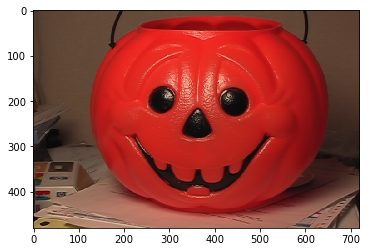
\includegraphics[width=0.6\linewidth]{images/1_a.png}
	\caption{The average pumpkin over 200 images.}
	\label{fig:avg_pumpkin}
	\end{figure}
	
	
	\paragraph{b)} The following code computes best basis using PCA with the snapshot method, and generates the eigenpumpkins. 
	
	\begin{lstlisting}
	# reshape data 
	X = pumpkin_mean_sub.reshape(-1, 480*720*3).T

	# first we get the eigenvectors of X.T*X and eigenvalues
	w, V = np.linalg.eig(X.T @ X)

	# arange eigenvectors based on values
	V = V[:, np.flip(np.argsort(w), axis=0)]
	w = w[np.flip(np.argsort(w), axis=0)]
	E = np.diag(np.sqrt((w > 0).astype(np.int8) * w))  # change negative data to 0

	# calculuate U
	U = X @ V @ np.linalg.pinv(E)
	print(U[:, 0]) # the first eigenvector
	
	# plot the eigenpumpkin
	fig = plt.figure(figsize=(12, 12))
	for i, ind in enumerate(list(range(4)) + list(range(100, 104))):
		x = np.copy(U[:, ind])
		x -= np.min(x)
		x = x / np.max(x)
		x = x.reshape(480, 720, 3)
		plt.subplot(4, 2, i+1)
		plt.axis('off')
		plt.title('Eigenpumpkin #%d' %(ind+1))
		plt.imshow(x)
	plt.show()
	
	# plot the eigenvalues
	plt.plot(w/200)
	plt.show()
	\end{lstlisting}
	
	The plot of eigenvalues are shown in figure~\ref{fig:evals}. Figure~\ref{fig:eig_pumpkin} shows the pictures of eigenpumpkins 1-4 and 101-104.\\
	Eigenpumpkins 1-4 have the shape of pumpkins, but eigenpumpkins 101-104 are almost all noise. This indicates that the most important features are already captured in the first few eigenvectors. This is also supported by the decrease of eigenvalues, which are the variance captured by each eigenvector. 
	\begin{figure}[h!]
	\centering
	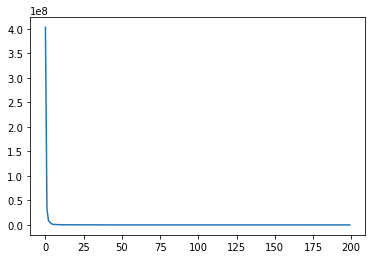
\includegraphics[width=0.7\linewidth]{images/1_b_eval.png}
	\caption{200 ordered eigenvalues.}
	\label{fig:evals}
	\end{figure}
	
	\begin{figure}[h!]
	\centering
	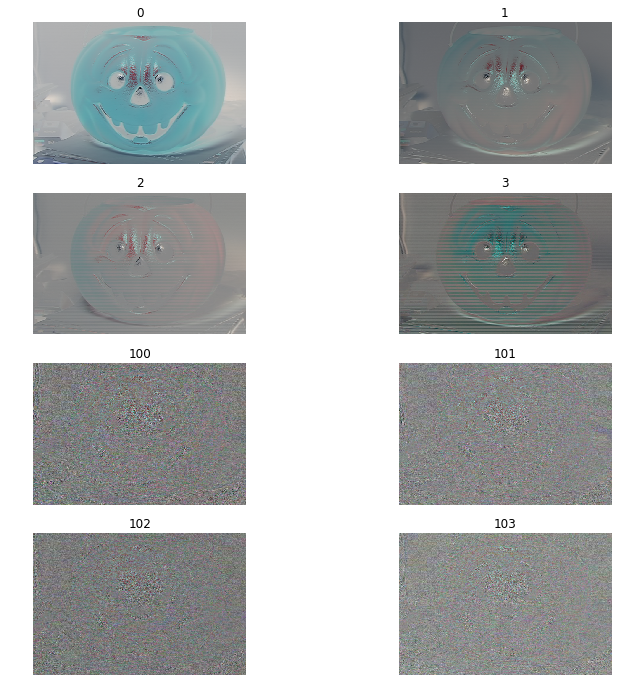
\includegraphics[width=\linewidth]{images/1_b_eigenpumpkin.png}
	\caption{Eigenpumpkins 1-4 and 101-104.}
	\label{fig:eig_pumpkin}
	\end{figure}
	
	
	\newpage
	\paragraph{c)} The following code uses svd to compute left singular vectors and singular values.
	\begin{lstlisting}
	U_svd, s, V = np.linalg.svd(X, full_matrices=False)
	
	# plot the squared singular values
	plt.plot(s**2/200)
	plt.show()
	\end{lstlisting}
		
	
	The eigenvectors from two different methods U\textunderscore svd and U are the same. 
	\begin{lstlisting}
	# U from snapshot method
	>>> U[:, 0]  # the first eigenvector
	array([ -4.06137377e-05,  -3.18043157e-05,  -9.74751095e-06, ..., -1.86172304e-03,  -1.55538031e-03,  -1.31720474e-03])
	>>> U_svd[:, 0]
	array([ -4.06137377e-05,  -3.18043157e-05,  -9.74751095e-06, ..., -1.86172304e-03,  -1.55538031e-03,  -1.31720474e-03])
	\end{lstlisting}
	
	Figure~\ref{fig:eval_svd} shows the squared singular values divided by the data size (200). This is the same with the eigenvalues computed from the snapshot method (figure~\ref{fig:evals}).
	\begin{figure}[ht!]
	\centering
	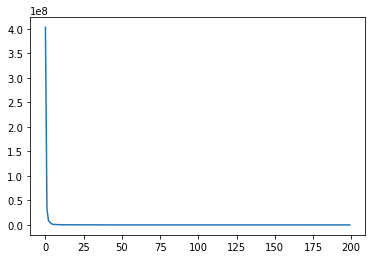
\includegraphics[width=0.7\linewidth]{images/1_c_eval.png}
	\caption{200 ordered eigenvalues.}
	\label{fig:eval_svd}
	\end{figure}
	
	
	\paragraph{d)} The following code computes the coefficients of the first two eigenvectors and plot them. 
	\begin{lstlisting}
	# compute the coefficients
	transformed_X = np.dot(X.T, U[:, :2])
	
	# plot the coefficients
	plt.figure(figsize=(8,8))
	plt.plot(transformed_X[:, 0], transformed_X[:, 1], '.')
	plt.xlabel('coeffient on first eigenvector')
	plt.ylabel('coeffient on second eigenvector')
	plt.show()
	\end{lstlisting}
	
	Figure~\ref{fig:coefficients} shows the coefficients of the pumpkin $(\alpha^{(\mu)}_1, \alpha^{(\mu)}_2)$ with respect to the PCA basis. 	
	\begin{figure}[ht!]
	\centering
	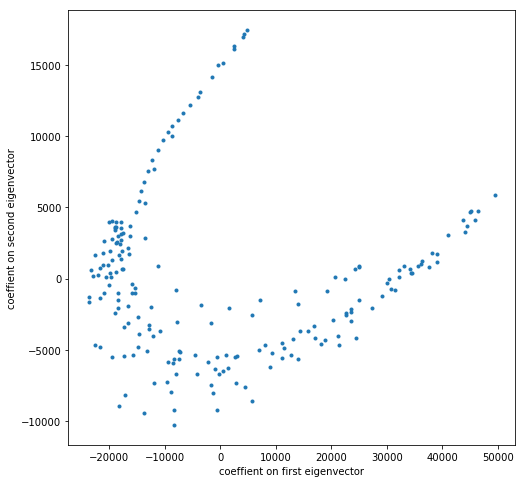
\includegraphics[width=0.9\linewidth]{images/1_d.png}
	\caption{The coefficients $(\alpha^{(\mu)}_1, \alpha^{(\mu)}_2)$}
	\label{fig:coefficients}
	\end{figure}
	
	
\newpage
\subsection{Problem 2}
First the following code was used to generate the data needed. 
\begin{lstlisting}
	import numpy as np
	import matplotlib.pyplot as plt
	import random

	def generate_data(P, M, N):
		res = [[0 for j in range(P)] for i in range(M)]
		for u in range(P):
			t = u*2*np.pi/P
			for m in range(M):
				x = m*2*np.pi/M
				tmp = [np.sin(k*(x-t))/k for k in range(1, N+1)]
				res[m][u] = np.mean(tmp)
    
		return np.array(res)
\end{lstlisting}


\paragraph{Part A} 
\subparagraph{} We can expand$f(x_m, t_\mu)$, and we get:
\begin{align*}
f(x_m, t_\mu) &= \frac{1}{N}\sum_{k=1}^{N}\frac{1}{k}\sin[k(x_m - t_\mu)] \\
&= \frac{1}{N}\sum_{k=1}^{N}\frac{1}{k}[\sin(kx_m)\cos(kt_\mu) + \cos(kx_m)\sin(kt_\mu)]
\end{align*}
Therefore each pattern is a linear combination of $\sin(kx_m), k \in [1,N]$ and $\cos(kx_m), k \in [1,N]$. In this example, $N=3$. Hence the rank is $2N=6$. 
\subparagraph{} The rank of the data matrix is 6, verified by program.
\begin{lstlisting}
	X = generate_data(64, 64, 3)
	np.linalg.matrix_rank(X)  # 6
\end{lstlisting}


\paragraph{Part B} SVD was used to compute a best basis. See the following code:
\begin{lstlisting}
	U, s, V = np.linalg.svd(X)  # calculate PCA eigenvectors
	
	# plot the first 6 basis
	fig = plt.figure(figsize=(12, 12))
	for i in range(6):
		plt.subplot(3,2, i+1)
		plt.plot(U[:, i])
		plt.tick_params(bottom='off', labelbottom='off')
		plt.title('#%d' %(i+1))
	plt.show()
\end{lstlisting}

The first 6 eigenvectors are shown in figure~\ref{fig:6evec}. The first 6 eigenvectors are sinusoidal patterns. 
\begin{figure}[h!]
\centering
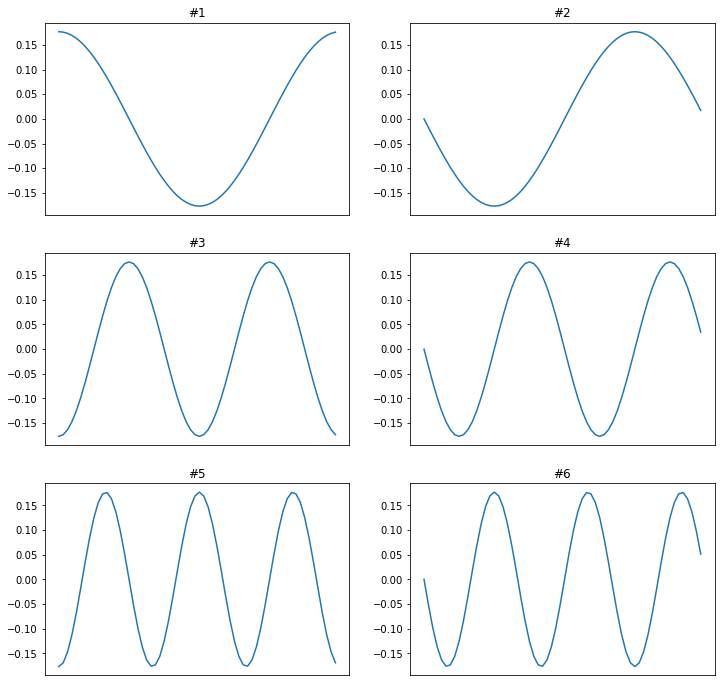
\includegraphics[width=\linewidth]{images/2_b.png}
\caption{First 6 eigenvectors}
\label{fig:6evec}
\end{figure}


\paragraph{Part C} A function create\textunderscore gappy\textunderscore single() is defined to generate a single gappy pattern with a certain percentage p of missing entries. 
\begin{lstlisting}
	def create_gappy_single(x, p):
		'''
		This function randomly generate a gappy pattern from x
		:param x: complete data x
		:param p: percentage of missing entries
		:return: gappy x filled with 0 and the mask
		'''
		n = int(x.shape[0] * p)  # the number of missing entries
		missing_ind = random.sample(range(x.shape[0]), n)
		m = [0 if i in missing_ind else 1 for i in range(x.shape[0])]
		m = np.array(m).reshape(x.shape)
    
		return x*m, m
\end{lstlisting}
The next function was defined to fix a single gappy pattern. 
\begin{lstlisting}
	def fix_single_pattern(U, m, x):
		'''
		This function takes a set of D good basis and fix one single gappy pattern
		:param U: first D basis from SVD left singular matrix
		:param x: gappy data which needs to be reconstructed
		:param m: gappy mask for x, 0 if missing data else 1
		:return: fixed x
		'''
		m = m.reshape(m.shape[0], 1)
		x = x.reshape(x.shape[0], 1) * m
		# first calculate alpha_hat (gappy_alpha)
		D = U.shape[1]
		M = np.array([[np.sum(i*j*np.squeeze(m)) for j in U.T] for i in U.T])  # M is a DxD matrix
		f = U.T@x
		gappy_alpha = np.linalg.inv(M)@f

		# gappy reconstruction
		g = U@gappy_alpha

		return x + g*(m == 0)
\end{lstlisting}
The following code was used to generate one single pattern and fix it. Errors were computed for each reconstruction as $\frac{\Vert{x-r}\Vert}{\Vert{x}\Vert}$ where $x$ is the actual pattern and $r$ is the reconstructed pattern.
\begin{lstlisting}
	def error_of_fixing(complete_x, p, U):
		xg, m = create_gappy_single(complete_x, p)
		x_fix = fix_single_pattern(U, m, xg)
		return np.linalg.norm(complete_x-x_fix) / np.linalg.norm(complete_x)

	# generate gappy pattern with different percentage of missing entries
	target_pattern = X[:, 0]
	errors = []
	for p in np.arange(0.05, 1.0, 1/64):
		errors.append(error_of_fixing(target_pattern, p, U[:, :6]))

	# plot reconstruction error
	plt.figure(figsize=(6,6))
	plt.plot(np.arange(0.05, 1.0, 1/64), errors)
	plt.xlabel('Percentage of missing entries')
	plt.ylabel('Reconstruction error')
	plt.show()
\end{lstlisting}
The reconstruction error plot is shown in figure~\ref{fig:reconstruct_error}. The algorithm is robust in the sense that it is able to completely reconstruct data until ~90\% entries are missing. 

\begin{figure}[h!]
\centering
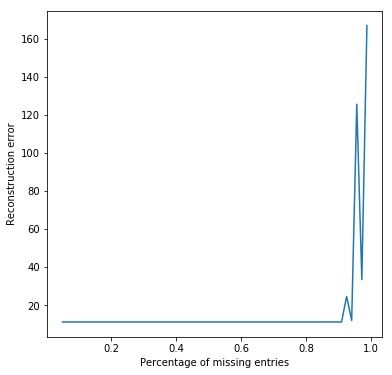
\includegraphics[width=0.6\linewidth]{images/2_c.png}
\caption{Reconstruction error with \% of missing entries}
\label{fig:reconstruct_error}
\end{figure}


\paragraph{Part D} The following code is used to repair the entire ensemble of corrupted patterns. Function create\textunderscore gappy\textunderscore ensemble() is used to generate an ensemble of gappy patterns. Function initial\textunderscore fix() is the zeroth fixing of the gappy data ensemble. Function general\textunderscore gappy\textunderscore fix() is the main function used to fix the ensemble gappy patterns. It returns the fixed data and the number of iterations. 
\begin{lstlisting}
	def create_gappy_ensemble(x, p):
		'''
		This function randomly generate an ensemble of gappy patterns from x
		:param x: complete data x
		:param p: percentage of missing entries
		:return: gappy x filled with 0 and the mask
	'''
	n = int(x.shape[0] * x.shape[1] * p)  # the number of missing entries
	missing_ind_flat = random.sample(range(x.shape[0] * x.shape[1]), n)
	m = np.ones(x.shape)
	for i in range(m.shape[0]):
		for j in range(m.shape[1]):
			if m.shape[1] * i + j in missing_ind_flat:
				m[i][j] = 0
				
				return x*m, m
			
	def initial_fix(x, m):
		'''
		:param x: gappy data
		:param m: mask having the same shape of x
		:return: initially fixed gappy data
	'''
	x = x.astype(np.float32)
	for i in range(m.shape[0]):
		known_mean = np.mean(x[i, m[i] != 0])
		x[i] = x[i] * m[i] + (m[i] == 0) * known_mean
		
		return x

	def general_gappy_fix(x, m, D, e, iter_max=100):
		'''
		This function fixes gappy data without known good basis
		:param x: gappy data that is already initially fixed
		:param m: mask having the same shape of x
		:param D: rank of non-gappy data
		:param e: stopping criterion
		:param iter_max: maximum number of iteration in case algorithm does not converge
		:return: fixed gappy data and the number of iterations
	'''
	U, s, V = np.linalg.svd(x)
	s_pre = s[:D]
	s_new = s_pre + e + 1 # initialize s_new so that the first iteration always run
	x_new = None
	for step in range(iter_max):
		if np.sqrt(np.linalg.norm(s_new**2 - s_pre**2)) <= e:
			break
		Ud = U[:, :D]
		x_new = []
		for i in range(x.shape[1]):
			x_new.append(fix_single_pattern(Ud, m[:, i], x[:, i]).squeeze())
			x_new = np.array(x_new).T
			x = x_new
			U, s, V = np.linalg.svd(x)
			s_pre = s_new
			s_new = s[:D]
			
			return x, step
\end{lstlisting}
The following code generates an ensemble of gappy patterns with 20\% missing entries. In this example, the reconstruction error is $2.5085403892e-06$. The missing entries in the first pattern have the original values of:\newline \textbf{[0.47291989,0.47351178,0.45281316,0.42166123,0.14760301,-0.03241118,\\-0.06297956,-0.12913006,-0.15589693,-0.17076234,-0.4062866,-0.09744129]},\\ and the reconstructed values are:\newline \textbf{[0.47291964,0.47351171,0.45281307,0.42166113,0.14760319,-0.03241126,\\-0.06297967,-0.12912921,-0.15589684,-0.17076257,-0.40628661,-0.09744129]}. This indicates that the algorithm is robust at repairing missing entries. 
\begin{lstlisting}
	xg, m = create_gappy_ensemble(X, 0.2)
	xg = initial_fix(xg, m)
	x_fixed, step = general_gappy_fix(xg, m, 6, 0.01)
	print(np.linalg.norm(X-x_fixed) / np.linalg.norm(X))
	print(X[m[:,0]==0,0])
	print(x_fixed[m[:,0]==0,0])
\end{lstlisting}

\paragraph{Part E} The following code is used to determine the relationship between the percentage of missing entries and the number of iterations required for data convergence. 
\begin{lstlisting}
	def convergence_rate_with_percent(p, max_iter):
		xg, m = create_gappy_ensemble(X, p)
		xg = initial_fix(xg, m)
		x_fixed, step = general_gappy_fix(xg, m, 6, 0.01, max_iter)
		
		return step

	conv_rates = []
	for p in np.arange(0.05, 0.8, 1/64):
		conv_rates.append(convergence_rate_with_percent(p, 200))
		
	# plot the result
	plt.figure(figsize=(6,6))
	plt.plot(np.arange(0.05, 0.8, 1/64), conv_rates)
	plt.xlabel('Percentage of missing entries')
	plt.ylabel('Number of iterations to converge')
	plt.show()
\end{lstlisting}
Figure~\ref{fig:convergence_step} shows the number of iterations with the percentage of missing entries. (Note: the maximum number of iterations allowed is 200 in case convergence takes a very long time to reach.)
\begin{figure}[h!]
\centering
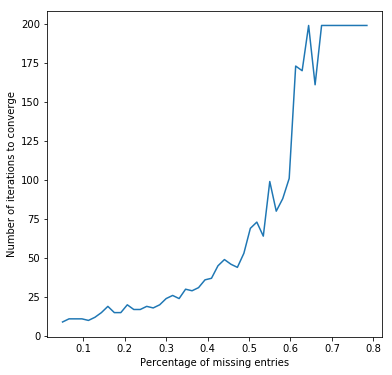
\includegraphics[width=0.7\linewidth]{images/2_e.png}
\caption{The number of iterations required for convergence.}
\label{fig:convergence_step}
\end{figure}

\end{document}









